\documentclass{article} % For LaTeX2e
\usepackage{nips15submit_e,times}
%\usepackage{hyperref}
%\usepackage{url}
\usepackage{amsmath}
%\newcommand\addtag{\refstepcounter{equation}\tag{\theequation}}
\usepackage{graphicx}

\title{Word and sentence embeddings\\
Sentence Classification with LSTMs/ConvNets}
\author{
Mario Ynocente Castro\\
Master MVA\\
ENS Cachan / Ecole Polytechnique\\
\texttt{mario.ynocente-castro@polytechnique.edu}
}

% The \author macro works with any number of authors. There are two commands
% used to separate the names and addresses of multiple authors: \And and \AND.
%
% Using \And between authors leaves it to \LaTeX{} to determine where to break
% the lines. Using \AND forces a linebreak at that point. So, if \LaTeX{}
% puts 3 of 4 authors names on the first line, and the last on the second
% line, try using \AND instead of \And before the third author name.

\newcommand{\fix}{\marginpar{FIX}}
\newcommand{\new}{\marginpar{NEW}}

\nipsfinalcopy % Uncomment for camera-ready version

\begin{document}
\maketitle

\section{Word and sentece embeddings with word2vec}

\subsection{Loading models}

\begin{enumerate}
    \item
    What is the total number of raw words found in the corpus?

    17,005,207 words.

    \item
    What is the number of words retained in the word2vec vocabulary
    (with default min\_count = 5)?

    71290 words.
\end{enumerate}

\subsection{Exploring the embedding space}

\begin{enumerate}
    \item
    What is the similarity between (’apple’ and ’mac’), between (’apple’ and ’peach’),
    between (’banana’ and ’peach’)? In your opinion, why are you asked about
    the three previous examples?

    \begin{itemize}
        \item
        Similarity between apple and mac: 0.567861632452

        \item
        Similarity between apple and peach: 0.178399832237

        \item
        Similarity between banana and peach: 0.688715470006
    \end{itemize}

    This illustrates that in this embedding space apple and mac are more similar than
    what apple and peach are even though both are fruits, in the case of banana and peach
    we do get a high similarity. This may happen because in the corpus the word apple
    is used more often as referring to the mark and less referring to the fruit, so it
    is more common to find it in the same context that the word mac.

    \item
    What is the closest word to the word 'difficult', for 'model' and 'model\_phrase'.
    Comment about the difference between model and model\_phrase. Find the three phrases
    that are closest to the word 'clinton'.

    \begin{itemize}
        \item
        Closest word to difficult for model: easy

        \item
        Closest word to difficult for model\_phrase: very\_difficult

        \item
        Difference between model and model\_phrase: model\_phrase was trained after
        preprocessing the tokens of the sentences in the corpus to group the ones
        that commonly occur together in phrases, model in contrast was trained
        directly on the individual tokens.

        \item
        Three phrases that are closest to clinton: bush, reagan and gore are the top
        and consist of only one token, the top consisting of two tokens are
        bill\_clinton, w\_bush and al\_gore.
    \end{itemize}

    \item
    Find the closest word to the vector "vect(france) - vect(germany) + vect(berlin)" and
    report its similarity measure.

    The closest word is 'paris' with similarity measure of 0.757699728012085

\newpage
    \item
    Explore the embedding space using these functions and report some interesting
    behaviour (of your choice)

    \begin{itemize}
        \item
        We can further confirm that the word apple is more frequently used (on the
        corpus) as related to the mark by checking which are its most similar words,
        which gives us: macintosh, atari, amiga, intel, ibm, pc
        \item
        We can make analogies like:
        \begin{itemize}
            \item science - scientist + mathematician $\approx$ mathematics
            \item science - scientist + physicist $\approx$ physics
            \item science - scientist + philosopher $\approx$ philosophy
            \item science - scientist + astronomer $\approx$ astronomy
            \item science - scientist + biologist $\approx$ humanities
        \end{itemize}
    \end{itemize}

\end{enumerate}

\subsection{Sentence embeddings}

\begin{enumerate}
    \item
    Report the closest sentence to the sentence with idx "777", and their
    similarity score.

    "gymnasts get ready for a competition ." with score 0.902949842134

    \item
    Report the 5 closest sentences to the sentence with idx "777", and the
    associated similarity scores.

    \begin{table}[h]
    \label{sample-table}
    \begin{center}
    \begin{tabular}{ll}
    \multicolumn{1}{c}{\bf Sentence} & \multicolumn{1}{c}{\bf Similarity score}
    \\ \hline \\
    gymnasts get ready for a competition . & 0.902949842134 \\
    a woman is getting ready to perform a song for the audience . & 0.890097422822 \\
    a runner in a competition want to go to the finish line . & 0.855536495002 \\
    men working to build a fence for customers . & 0.851471676783 \\
    a man prepares to give a speech for a television audience . & 0.849476121272 \\
    \end{tabular}
    \end{center}
    \end{table}
\end{enumerate}

\subsection{IDF weighted sentence embeddings}

\begin{enumerate}
    \item
    Report the IDF score of the word "the", the word "a", and the word "clinton".

    The word "the" has a score of 0.867762351618

    The word "a" has a score of 0.473266274881

    The word "clinton" doesn't have an IDF score since it's not present in the data.

    \item
    Report the closest sentence to sentence with idx 777.

    The closest sentence is "gymnasts get ready for a competition ." with a score of 0.897237646962.
\end{enumerate}

\section{Simple LSTM for Sequence Classification}

\begin{enumerate}
    \item
    What is the (minibatch) shape of:

    \begin{itemize}
        \item
        the input of the embedding layer: $32 \times 80$
        \item
        the input of the LSTM layer: $32 \times 80 \times 32$
        \item
        the output of the LSTM layer $32 \times 64$
    \end{itemize}

    \item
    Report the number of parameters of the model with the standard set of hyper-parameters.
    Report also the number of sentences in the training set. In standard statistics,
    a rule of thumb is to have less parameters than samples in your dataset.
    How do you think it’s possible to train a model that has so many parameters
    compared to this number of samples?

    \begin{itemize}
        \item
        Number of hyper-parameters: 480000
        \item
        Number of sentences in the training set: 35000
        \item
        We are adding some regularization to the model, in this particular case
        we use dropout, which can be seen as training multiple similar models
        with some constraints of weight sharing.
    \end{itemize}

    \item
    For a single sentence, the LSTM has states $h_1, \ldots, h_T$ where $T$ is
    the number of words in the sentence. The sentence embeddings that is fed to
    the classifier is thus computed as $f(h_1, \ldots, h_T)$. What is the exact
    form of $f(h_1, \ldots, h_T)$ used in the python script?

    Keras implements LSTM according to the following recurrent formulas:

    \begin{center}
        $f_t = \sigma(W_f x_t + U_f h_{t - 1} + b_f), i_t = \sigma(W_i x_t + U_i h_{t - 1} + b_i)$

        $C_t = f_t C_{t - 1} + i_t \tanh(W_c x_t + U_c h_{t - 1} + b_c)$

        $o_t = \sigma(W_o x_t + U_o h_{t - 1} + b_o), h_t = o_t \tanh(C_t)$
    \end{center}

    If the flag return\_sequences is set to False (which is the default) then
    $f(h_1,\ldots,h_T) = h_T$, if it is True then $f(h_1,\ldots,h_T) = [h_1; \ldots; h_T]$.

    \item
    Plot the evolution of the train and valid accuracy per epoch, and write the
    test errors that you obtain.

    \begin{figure}[ht]
    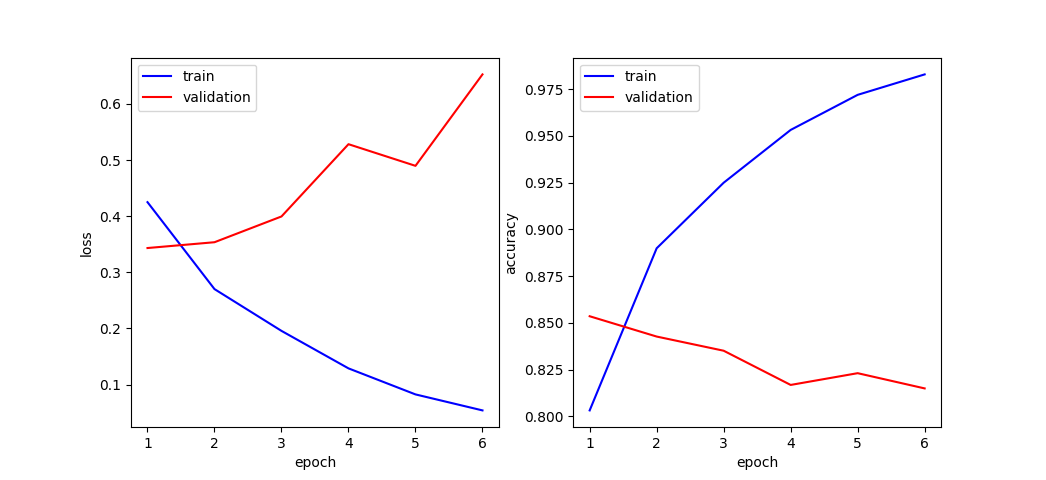
\includegraphics[width=\textwidth,height=\textheight,keepaspectratio]{img/lstm_no_dropout_loss_acc.png}
    \caption{Evolution of the loss and accuracy with no dropout.}
    \end{figure}

    \begin{figure}[ht]
    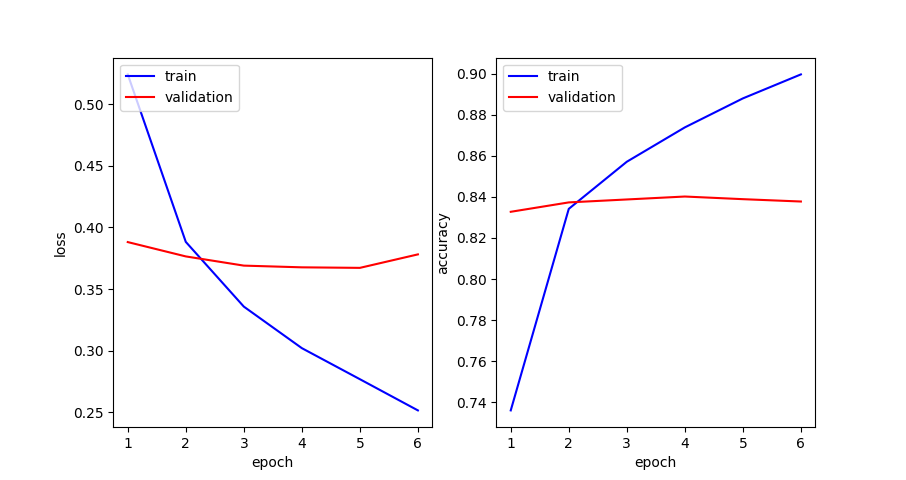
\includegraphics[width=\textwidth,height=\textheight,keepaspectratio]{img/lstm_dropout_loss_acc.png}
    \caption{Evolution of the loss and accuracy with dropout.}
    \end{figure}

    \begin{itemize}
        \item
        Results without dropout: loss = 0.656337736861, error = 18.0866666698\%

        \item
        Results with dropout: loss = 0.377996407843, error = 16.606666666699998\%
    \end{itemize}

    \item
    Explain what is the difference between SGD and Adam.

    The difference is that Adam uses an exponentially
    decaying average of the past gradients and also divides this by another similarly
    calculated average, but this time of the sum of squares of the terms in the
    gradient, which has the effect of decreasing the learning rate of the parameters
    that have been updated the most.
\end{enumerate}

\section{Simple ConvNet for Sequence Classification}

\begin{enumerate}
    \item
    Report the results (test loss and test error) that you obtain.

    Loss = 0.361414234543

    Error = 16.3333333365\%

    \begin{figure}[ht]
    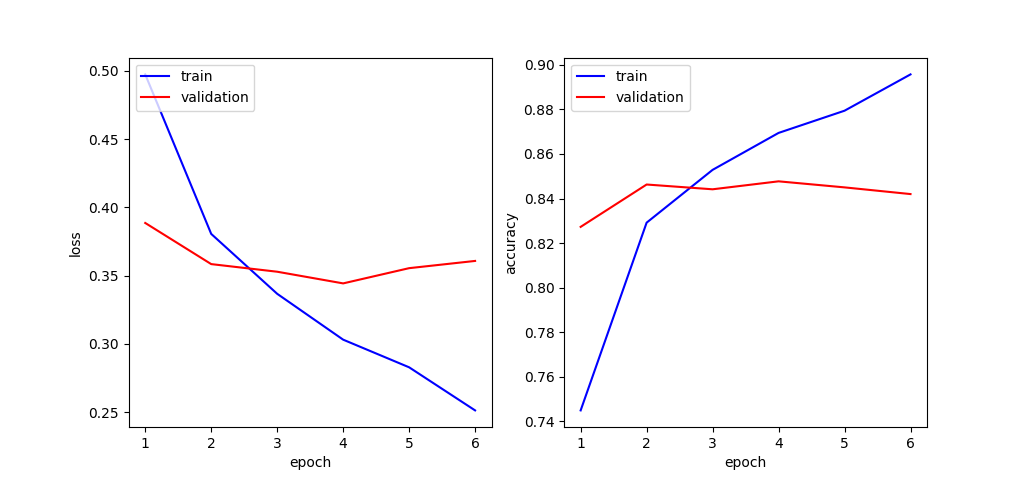
\includegraphics[width=\textwidth,height=\textheight,keepaspectratio]{img/cnn_loss_acc.png}
    \caption{Evolution of the loss and accuracy with 1D Convolution.}
    \end{figure}

    \item
    What is the input and output shape of Convolution1D?

    Input's shape: $32 \times 80 \times 16$

    Output's shape: $32 \times 78 \times 250$

    \item
    Build a model where on top of the convolution, you have an LSTM. It means
    that the input of the LSTM will be the output of your ConvNet. Run the model
    with the best parameters you find. Report your best results.

    Loss = 0.338560722351

    Error = 14.673333333299998\%

    \begin{figure}[ht]
    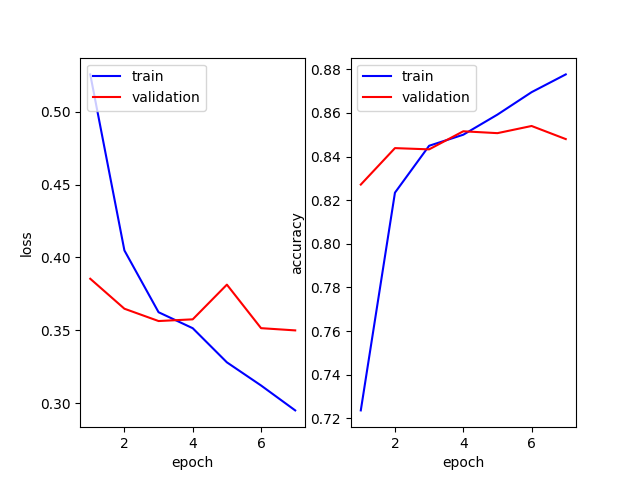
\includegraphics[width=\textwidth,height=\textheight,keepaspectratio]{img/cnn_lstm_loss_acc.png}
    \caption{Evolution of the loss and accuracy with LSTM on top of 1D Convolution.}
    \end{figure}
\end{enumerate}

\end{document}
